\documentclass[a4paper,14pt,ukrainian]{extreport}

\usepackage{extsizes}
\usepackage{titlesec}
\usepackage{cmap}
\usepackage[T2A]{fontenc}
\usepackage[utf8]{inputenc}
\usepackage[ukrainian]{babel}

\usepackage{pscyr}
\usepackage{graphicx}
\usepackage{amssymb,amsfonts,amsmath,amsthm}
\usepackage{indentfirst}
\usepackage[usenames,dvipsnames]{color}
\usepackage{makecell}
\usepackage{multirow}
\usepackage{ulem}
\usepackage{tocloft}
\usepackage{import}
\usepackage{lastpage}
\usepackage{etoolbox}
\usepackage{listings}


\def\figureautorefname{рис.}

\usepackage{geometry}
\geometry{left=1.5cm}
\geometry{right=1cm}
\geometry{top=1.5cm}
\geometry{bottom=2cm}

\clubpenalty=10000
\widowpenalty=10000
\begin{document}
\lstset{
    numbers=left,
    tabsize=4,
    breaklines=true,
    title=\lstname,
    basicstyle=\footnotesize, % \ttfamily,
}
\begin{titlepage}
    \begin{center}

    \centering \large Національный технічний університет України \\ "Київський політехнічний інститут"
    \vfill
    \textsc{\Large Лабораторна робота}\\[0.5cm]

    % Title
    { \huge Тема: Дослідження дисциплін обслуговування заявок при обмежених ресурсах  }\\[0.4cm]
    \vfill

    % Author and supervisor
    \begin{flushright} 
        \Large \emph{Виконав:}\\
        Радер Роман\\
        залікова книжка: 215\\
        група \textsc{ІО-02}\\
    \end{flushright}
    \vfill
    % Bottom of the page
    {\large Київ 2013}

    \end{center}
\end{titlepage}

%----------------------------
Варіант: $15 \% 16 + 1 = 16$ 16. Змішаний алгоритм. FIFO + АП


Вхідні дані: тривалість кванту часу, кількість черг, кількість квантів часу для кожної черги, інтенсивність задач та інтенсивність задач з абсолютним пріоритетом.

Середній час очікування в черзі від інтенсивності заявок:

\begin{figure}[H]
Час чекання в черзі від інтенсивності:

  \includegraphics[width=0.85\textwidth]%
    {waiting_time.png}
\end{figure}

\begin{figure}[H]
Час чекання в черзі від довжини задачі:

  \includegraphics[width=0.85\textwidth]%
    {waiting_by_duration_with_queues.png}
\end{figure}

\begin{figure}[H]
Час простою від інтенсивності заявок:

  \includegraphics[width=0.85\textwidth]%
    {idle_time.png}
\end{figure}

\begin{figure}[H]
Кількість опрацьованих задач від часу чекання:

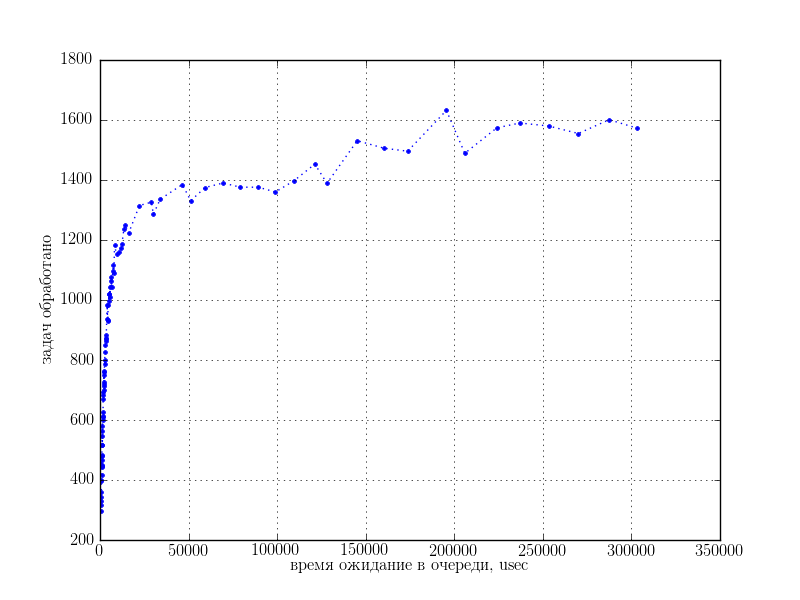
\includegraphics[width=0.85\textwidth]
    {tasks_count_by_waiting_time.png}
\end{figure}

\begin{figure}[H]
Середній час очікування задач абсолютного приорітету в черзі від інтенсивності заявок:

  \includegraphics[width=0.85\textwidth]%
    {waiting_time_AP.png}
\end{figure}

\lstset{language=Python,
   breaklines=true,
   extendedchars=\true,
   basicstyle=\footnotesize\ttfamily}
\linespread{1}
\lstinputlisting{l3.py}

\end{document}
